\documentclass[10pt,t,svgnames]{beamer}

\usetheme{metropolis} % use metropolis theme

\usepackage{../solarized}         % use solarized themed listings
\usepackage{../stack}             % use the tikzstack environment
\usepackage{appendixnumberbeamer} % do not number appendix frames
\usepackage[scale=3]{ccicons}     % creative commons icons

% fix-up the handling of the notes pages
\ifnotes
  \hypersetup{final}
  \usepackage{pgfpages}
  \setbeamertemplate{note page}[plain]
  \setbeameroption{show notes on second screen=right}
  \AtBeginNote{%
    \let\enumerate\itemize%
    \let\endenumerate\enditemize%
  }
\fi

% overrides default description environment
\newlength\wideleftmargin{}
\newlength\tightleftmargin{}
\newlength\diffleftmargin{}
\setlength\wideleftmargin{6em}    % controls location of term (> is more left)
\setlength\tightleftmargin{1.5em} % controls location of description (same)
\setlength\diffleftmargin{\dimexpr\wideleftmargin-\tightleftmargin}
\makeatletter
\providecommand{\nextline}{
  \setlength\labelwidth{\tightleftmargin}
  \setlength\leftmargin{\tightleftmargin}
  \advance\linewidth\diffleftmargin{}
  \advance\@totalleftmargin-\diffleftmargin{}
  \parshape\@ne\@totalleftmargin\linewidth{}
  \setlength\itemsep{1.5ex}
}
\makeatother
\let\origdescription\description
\let\endorigdescription\enddescription
\renewenvironment{description}{\origdescription\nextline}{\endorigdescription}

%-------------------------------------------------------------------------------

\usepackage{tabularx}   % tables
\usepackage{subcaption} % subfigures
\usepackage{tikz}       % tikz
\usetikzlibrary{decorations.pathreplacing,positioning}

\tikzset{
  annotation/.style={
    remember picture,
    overlay,
    every edge/.append style={
      ->,
      thick,
      >=stealth,
      DimGray,
      dashed,
      thick,
    },
    every node/.append style={
      draw,
      align=center,
      minimum height=10pt,
      color=DimGray,
      text=fg,
      thin,
      rounded corners,
      text width=.25\linewidth,
    },
    group/.style = {
      decoration={
        brace,
        mirror,
        raise=5pt,
      },
      thick,
      color=DimGray,
      decorate,
    },
  }
}

\title{C programming language}
\date{}
\author{College of Saint Benedict \& Saint John's University}
\begin{document}
  \maketitle

  \begin{frame}{origins}
  %{{{1
    \vspace{3ex}
    \begin{columns}
      \begin{column}{.38425\textwidth}
        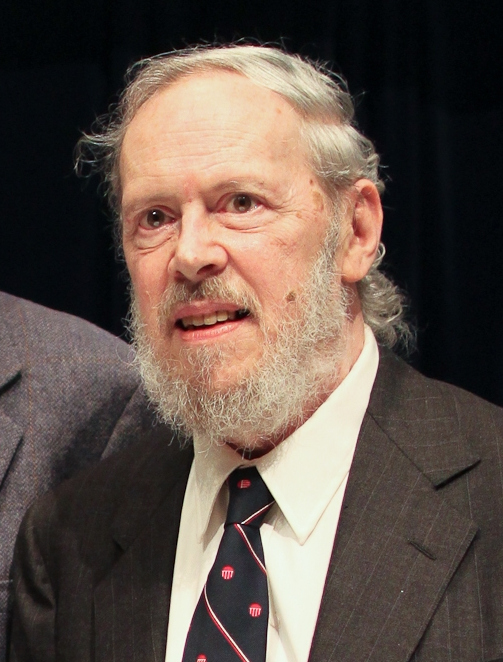
\includegraphics[width=\textwidth]{Dennis_Ritchie_2011.jpg}\\
        \hfill \tiny{\href{https://en.wikipedia.org/wiki/Dennis\_Ritchie\#/media/File:Dennis\_Ritchie\_2011.jpg}{Dennis~Ritchie~in~2011}~/~\href{http://creativecommons.org/licenses/by-sa/2.0}{CC~BY~2.0}}
      \end{column}
      \begin{column}{.51575\textwidth}
        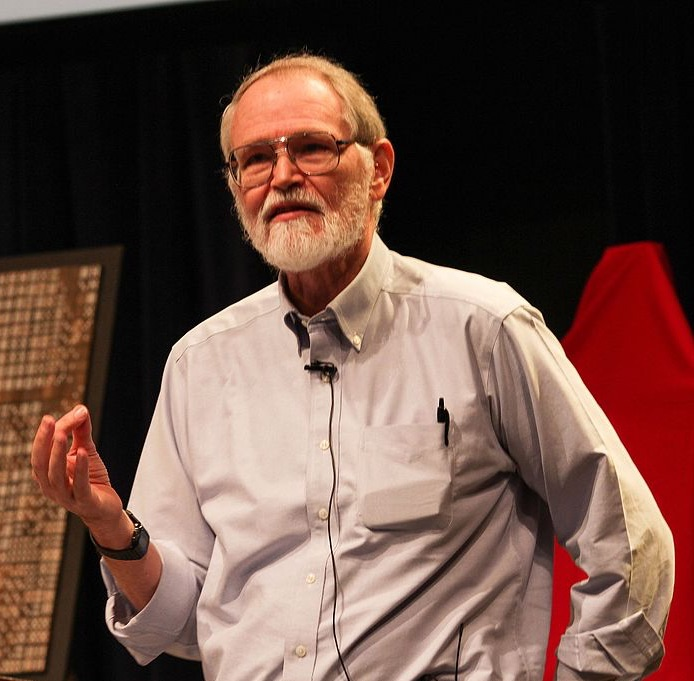
\includegraphics[width=\textwidth]{Brian_Kernighan_2012.jpg}\\
        \hfill \tiny{\href{https://en.wikipedia.org/wiki/Brian\_Kernighan\#/media/File:Brian\_Kernighan\_in\_2012\_at\_Bell\_Labs\_1.jpg}{Brian~Kernighan~in~2012}~/~\href{http://creativecommons.org/licenses/by-sa/2.0}{CC~BY~2.0}}
      \end{column}
    \end{columns}

    \note[item]{Dennis Ritchie and Brian Kernighan creators of C circa 1972}
    \note[item]{TODO: more thorough history}
  %}}}1
  \end{frame}

  \begin{frame}[fragile]{hello, world}
  %{{{1
    \begin{codeblock}
    /* file: helloworld.c */

    ###include## $$<stdio.h>$$

    int main() {
      printf([["hello, world]]%%\n%%[["]]);
      return $$0$$;
    }
    \end{codeblock}

    \begin{termblock}
    $ gcc -o helloworld helloworld.c
    $ ./helloworld
    hello, world
    \end{termblock}

    \note{
      \begin{itemize}
        \item Remind students that not everyone has same background in C ---
          those with experience can help those without
      \end{itemize}
      \begin{itemize}
        \item The tradition of using the phrase "Hello, world!" as a test
          message was influenced by an example program in the seminal book
          \emph{The C Programming Language}
        \item Every statement in C exists in a function, starting with
          \texttt{main}
        \item Refresh students memory on the \emph{traditional} compilation
          process
      \end{itemize}
    }
  %}}}1
  \end{frame}

  \begin{frame}[fragile]{global variables}
  %{{{1
    \begin{scriptsize}
      \begin{codeblock}
      // file: figure2-4.c
      // Stan Warford
      // A nonsense program to illustrate global variables

      ###include## $$<stdio.h>$$

      char ch;
      int j;

      int main() {
        scanf([["]]%%%c%%[[ ]]%%%d%%[["]], &ch, &j);
        j += $$5$$;
        ch++;
        printf([["]]%%%c\n%d\n%%[["]], ch, j);
        return $$0$$;
      }
      \end{codeblock}
    \end{scriptsize}

    \begin{scriptsize}
      \begin{termblock}
      $ gcc -o figure2-4 figure2-4.c
      $ ./figure2-4
      M 419
      N
      424
      \end{termblock}
    \end{scriptsize}

    \note{
      \begin{itemize}
        \item Every C variable has three attributes:
          \begin{description}
            \item[name]  an identifier determined arbitrarily by the programmer
            \item[type]  specifies the kind of values it can have
            \item[value]
          \end{description}
        \item In C, variable declaration only reserves storage for the value;
          nothing can be assumed about the initial value
      \end{itemize}
      \begin{itemize}
        \item What would you expect for input '\texttt{Z~-3}'?
        \item What would you expect for input '\texttt{9~a}'?
        \item What would you expect for input
          '\texttt{\textasciitilde~2147483643}'?
      \end{itemize}
    }
  %}}}1
  \end{frame}

  \begin{frame}[fragile]{program breakdown}
  %{{{1
    \vspace{1\baselineskip}

    \begin{scriptsize}
      \begin{codeblock}[escapechar=!,xleftmargin=.45\linewidth,firstnumber=5]
      ###include## $$<stdio.h>$$!\tikz[remember picture] \coordinate (f);!

      !\tikz[remember picture] \coordinate (a);!char ch;
      !\tikz[remember picture] \coordinate (b);!int j;

      int main() {!\tikz[remember picture] \coordinate (c);!
        !\tikz[remember picture] \coordinate (i);!scanf([["]]%%%c%%[[ ]]%%%d%%[["]], &ch, &j);!\tikz[remember picture] \coordinate (g);!
        j += $$5$$;
        !\tikz[remember picture] \coordinate (d);!ch++;
        !\tikz[remember picture] \coordinate (h);!printf([["]]%%%c\n%d\n%%[["]], ch, j);!\tikz[remember picture] \coordinate (j);!
        return $$0$$;!\tikz[remember picture] \coordinate (e);!
      }
      \end{codeblock}
        \begin{tikzpicture}[annotation]
          \only<1>{
            \node[] at ([shift=({19.5em,.625ex})]c) (C) {C programs ALWAYS start execution with the \texttt{main} function};
            \node[] at ([shift=({20em,.625ex})]e) (E) {returning from \texttt{main} ends the program};
            \draw (C.west) edge ([shift=({.4em,.625ex})]c);
            \draw (E.west) edge ([shift=({.4em,.625ex})]e);
          }
          \only<2>{
            \draw[group] ([shift=({.4em,1.65ex})]a) -- node[left=4.5em] (AB) {global variables are declared here --- outside of any function} ([shift=({.4em,-.4ex})]b);
            \node[] at ([shift=({-11em,.625ex})]d) (D) {characters in C are treated internally like signed integers};
            \draw (AB.east) edge ([xshift=3em]AB.east);
            \draw (D.east) edge ([shift=({-.4em,.625ex})]d);
          }
          \only<3>{
            \node[] at ([shift=({16em,.625ex})]f) (F) {correct headers must be included to access library functions};
            \node[] at ([shift=({-11em,.625ex})]h) (H) {print data to \texttt{stdout} (the terminal)};
            \node[] at ([shift=({-11em,.625ex})]i) (I) {read data from \texttt{stdin} (the terminal)};
            \node[] at ([shift=({11em,-3.625ex})]g) (GJ) {\texttt{scanf} and \texttt{printf} are both library functions declared in \texttt{stdio.h}};
            \draw (F.west) edge ([shift=({.4em,.625ex})]f);
            \draw (GJ.west) edge ([shift=({.4em,.625ex})]g);
            \draw (GJ.west) edge ([shift=({.4em,.625ex})]j);
            \draw (H.east) edge ([shift=({-.4em,.625ex})]h);
            \draw (I.east) edge ([shift=({-.4em,.625ex})]i);
          }
          \only<4>{
            \node[] at ([shift=({11em,.625ex})]g) (G) {\texttt{\&} is the address of operator --- \texttt{scanf} expects the address of the variables where the data will be stored};
            \draw (G.west) edge ([shift=({.4em,.625ex})]g);
          }
        \end{tikzpicture}
      \end{scriptsize}

      \note[item]<3>{C has no ``built-in'' functions; however, it does have a
        standard library that includes many useful utility functions.}
      \note[item]<4>{address here means the location in memory}
  %}}}1
  \end{frame}

  \begin{frame}{memory model --- part i}
  %{{{1
    \begin{description}
      \item[global variables] \hfill \\ declared outside of any function and
        remain in place throughout the execution of the entire program. they are
        stored at a fixed location in memory.
      \item[local variables] \hfill \\ declared within a function and come into
        existence when the function is called and cease to exist when the
        function terminates. they are stored on the run-time stack.
    \end{description}

    \vspace{1\baselineskip}

    \begin{figure}
      \centering
      \begin{subfigure}[b]{.30\textwidth}
        \centering
        \begin{tikzstack}[bg]
          \begin{stack}{west}
            % global variables
            \variables{j/424,ch/N}
          \end{stack}
        \end{tikzstack}
        \caption{Fixed location.}
      \end{subfigure}
      \quad
      \begin{subfigure}[b]{.30\textwidth}
        \centering
        \begin{tikzstack}[fg]
          \begin{stack}{east}
            % stack variables
            \variables{retVal/0,retAddr/ra0}
            % stack frames
            \frames{0/2}
          \end{stack}
        \end{tikzstack}
        \caption{Run-time stack.}
      \end{subfigure}
    \end{figure}

    \note{
      \begin{itemize}
        \item I will be using graphical notation consistent with that of the
          book.
        \item In this case, (a) and (b) represent the state of relevant memory
          for the previous program just before it terminates, i.e., in the
          process of executing line 15.
      \end{itemize}
    }
  %}}}1
  \end{frame}

  \begin{frame}{run-time stack a.k.a. ``the stack''}
  %{{{1
    \begin{description}
      \item[run-time stack] \hfill \\ stores information about the active
        functions of a C program, including:
        \begin{itemize}
          \item return value,
          \item actual parameters,
          \item return address, and
          \item local variables
        \end{itemize}
        in that order.
    \end{description}

    \begin{onlyenv}<2>
      \vspace{.5\baselineskip}

      \begin{figure}
        \centering
        \begin{subfigure}[b]{.30\textwidth}
          \centering
          \begin{tikzstack}[fg]
            \begin{stack}{west}
              % stack variables
              \variables{retVal/0,retAddr/ra0,j/424,ch/N}
              % stack frames
              \frames{0/4}
            \end{stack}
          \end{tikzstack}
          \caption{}
        \end{subfigure}
        \quad
        \begin{subfigure}[b]{.30\textwidth}
          \centering
          \begin{tikzstack}[fg]
            \begin{stack}{west}
              % stack variables
              \variables{ch/N,j/424,retAddr/ra0,retVal/0}
              % stack frames
              \frames{0/4}
            \end{stack}
          \end{tikzstack}
          \caption{}
        \end{subfigure}
      \end{figure}
    \end{onlyenv}

    \note[item]{
      I will not distinguish between functions and procedures
      \begin{itemize}
        \item functions that have no return value, i.e., return type
          \texttt{void}, just omit the first bullet point
      \end{itemize}
    }
    \note[item]{each program has one stack}
    \note[item]<2>{which visualization is correct, had \texttt{ch} and
      \texttt{j} been declared as local variables instead of global?}
  %}}}1
  \end{frame}

  \begin{frame}[fragile]{functions}
  %{{{1
    \vspace{2.5\baselineskip}
    % FIXME ??? why is this needed ???
    \only<1>{\vspace{-.1125\baselineskip}}

    \begin{scriptsize}
      % FIXME ??? gobble=2 not working in options for this codeblock ???
      \begin{codeblock}[escapechar=!,xleftmargin=.45\linewidth]
      !\tikz[remember picture] \coordinate (a);!void print_bar!\tikz[remember picture] \node [] (b) {};
      !(int!\tikz[remember picture] \node [] (c){};!n) {
        int k;
        for (k=$$0$$; k<n; k++) {
          printf([["*"]]);
        }
        printf([["]]%%\n%%[["]]);
      }
      \end{codeblock}
      \begin{tikzpicture}[annotation]
        \node[] at ([shift=({-10em,.625ex})]a) (A) {return value type};
        \node[above left=.35cm and -.75cm of b] (B) {function name};
        \node [above right=0.10cm and -1.35cm of B] (C) {list of formal parameters};
        \draw (A.east) edge ([shift=({-.4em,.625ex})]a);
        \draw (B.south) + (0, 0) coordinate(x1) edge (x1|-b.north);
        \draw (C.south) + (0, 0) coordinate(x3) edge (x3|-c.north);
      \end{tikzpicture} 
    \end{scriptsize}

    \vspace{-1\baselineskip}

    \begin{onlyenv}<2>
      \begin{scriptsize}
        \begin{codeblock}[escapechar=!,xleftmargin=.45\linewidth,gobble=4]
          !\tikz[remember picture] \coordinate (a);!int fact(int n) {
            int f, j;
            f = $$1$$;
            for (j=$$1$$; j<=n; j++) {
              f *= j;
            }
            return f;!\tikz[remember picture] \coordinate (b);!
          }
        \end{codeblock}
        \begin{tikzpicture}[annotation]
          \node[] at ([shift=({-10em,.625ex})]a) (A) {return value type};
          \node[] at ([shift=({20em,.625ex})]b) (B) {type of \texttt{<expr>} must
            match return type of function};
          \draw (A.east) edge ([shift=({-.4em,.625ex})]a);
          \draw (B.west) edge ([shift=({.4em,.625ex})]b);
        \end{tikzpicture} 
      \end{scriptsize}
    \end{onlyenv}
  %}}}1
  \end{frame}

  % FIXME fix the order of return address and parameters on the stack
  \begin{frame}[fragile]{functions --- call-by-value}
  %{{{1
    \begin{columns}
      \begin{column}{.65\textwidth}
        \vspace{-15em} % FIXME ??? why is this needed ???
        \begin{scriptsize}
          % FIXME Use moredelim from listing package to achieve this effect
          % without providing each animation separately
          \begin{onlyenv}<1>
            \begin{codeblock}[firstnumber=5, gobble=8]
              int fact(int n) {
                int f, j;
                f = $$1$$;
                for (j=$$1$$; j<=n; j++) {
                  f *= j;
                }
                return f;
              }

              int main() {
                int n;
                scanf([["]]%%%d%%[["]], &n);
                printf([["]]%%%d\n%%[["]], fact(n)); // ra1
                return $$0$$;
              }
            \end{codeblock}
          \end{onlyenv}
          \begin{onlyenv}<2>
            \begin{codeblock}[firstnumber=5, gobble=8]
              **int fact(int n) {
                int f, j;
                f = 1;
                for (j=1; j<=n; j++) {
                  f *= j;
                }
                return f;
              }

              int main() {
                int n;**
                scanf([["]]%%%d%%[["]], &n);**
                printf("%d\n", fact(n)); // ra1
                return 0;
              }**
            \end{codeblock}
          \end{onlyenv}
          \begin{onlyenv}<3>
            \begin{codeblock}[firstnumber=5, gobble=8]
              **int fact(int n) {
                int f, j;
                f = 1;
                for (j=1; j<=n; j++) {
                  f *= j;
                }
                return f;
              }

              int main() {
                int n;
                scanf("%d", &n);**
                printf([["]]%%%d\n%%[["]], fact(n));** // ra1
                return 0;
              }**
            \end{codeblock}
          \end{onlyenv}
          \begin{onlyenv}<4>
            \begin{codeblock}[firstnumber=5, gobble=8]
              **int fact(int n) {
                int f, j;
                f = 1;
                for (j=1; j<=n; j++) {
                  f *= j;
                }
                return f;
              }

              int main() {
                int n;
                scanf("%d", &n);
                printf("%d\n", **fact(n)**); // ra1
                return 0;
              }**
            \end{codeblock}
          \end{onlyenv}
          \begin{onlyenv}<5>
            \begin{codeblock}[firstnumber=5, gobble=8]
              **int fact(int n) {
                int f, j;
                f = 1;
                for (j=1; j<=n; j++) {
                  f *= j;
                }
                **return f;**
              }

              int main() {
                int n;
                scanf("%d", &n);
                printf("%d\n", fact(n)); // ra1
                return 0;
              }**
            \end{codeblock}
          \end{onlyenv}
          \begin{onlyenv}<6>
            \begin{codeblock}[firstnumber=5, gobble=8]
              **int fact(int n) {
                int f, j;
                f = 1;
                for (j=1; j<=n; j++) {
                  f *= j;
                }
                return f;
              }

              int main() {
                int n;
                scanf("%d", &n);**
                printf([["]]%%%d\n%%[["]], fact(n));** // ra1
                return 0;
              }**
            \end{codeblock}
          \end{onlyenv}
          \begin{onlyenv}<7>
            \begin{codeblock}[firstnumber=5, gobble=8]
              **int fact(int n) {
                int f, j;
                // f = 1;
                for (j=1; j<=n; j++) {
                  f *= j;
                }
                return f;
              }

              int main() {
                int n;
                scanf("%d", &n);
                printf("%d\n", fact(n));
                scanf("%d", &n);**
                printf([["]]%%%d\n%%[["]], fact(n));** // ra1
                return 0;
              }**
            \end{codeblock}
          \end{onlyenv}
        \end{scriptsize}
      \end{column}

      \begin{column}{.35\textwidth}
        \vspace*{5em}
        \begin{tikzstack}[fg]
          \draw[use as bounding box,bg] (0,0) rectangle (3,15);
          \begin{stack}{east}
            % stack variables
            \only<1>{\variables{retVal/,retAddr/ra0,n/}}
            \only<2>{\variables{retVal/,retAddr/ra0,n/3}}
            \only<3>{\variables{retVal/,retAddr/ra0,n/3}}
            \only<4>{\variables{retVal/,retAddr/ra0,n/3,retVal/,n/3,retAddr/ra1,f/,j/}}
            \only<5>{\variables{retVal/,retAddr/ra0,n/3,retVal/6,n/3,retAddr/ra1,f/6,j/4}}
            \only<6>{\variables{retVal/,retAddr/ra0,n/3,/6,/3,/ra1,/6,/4}}
            \only<7>{\variables{retVal/,retAddr/ra0,n/3,retVal/6,n/3,retAddr/ra1,f/6,j/4}}
            % stack frames
            \only<1>{\frames{0/3}}
            \only<2>{\frames{0/3}}
            \only<3>{\frames{0/3}}
            \only<4>{\frames{0/3,3/5}}
            \only<5>{\frames{0/3,3/5}}
            \only<6>{\frames{0/3}}
            \only<7>{\frames{0/3,3/5}}
          \end{stack}
        \end{tikzstack}
      \end{column}
    \end{columns}

    \note[item]<1>{you will have to reconcile this example a little bit with the
      book, since the solution is written slightly different}
    \note[item]<1>{assume nothing about values that are blank --- they are not 0}
    \note[item]<2>{assume the user inputs the number 3}
    \note[item]<3>{this statement requires that we evaluate the expression
      \texttt{fact(n)}}
    \note[item]<4>{\texttt{fact(n)} is a function call, so a new stack frame is
      pushed on to the stack in the sequence described before:
      \begin{itemize}
        \item return value
        \item actual parameters
        \item return address
        \item local variables
      \end{itemize}
    }
    \note[item]<5>{the state of the run-time stack after \texttt{fact} function
      has completed, but before returning}
    \note[item]<6>{after \texttt{fact} returns, its stack frame is deallocated,
      however, the values computed are still in memory --- since return value is
      always first thing pushed on to stack, the main function knows exactly
      where to find the value returned by \texttt{fact(n)}}
    \note[item]<7>{assume the the first call to \texttt{fact} got lucky and the
      value 1 happended to be in the memory cell designated to the variable
      \texttt{f}, so that the calculation worked out correctly}
    \note[item]<7>{this would be the state of the stack at the beginning of
      execution of the second call to \texttt{fact}}
  %}}}1
  \end{frame}

  \begin{frame}[fragile]{functions --- call-by-``reference''}
  %{{{1
    \begin{columns}
      \begin{column}{.65\textwidth}
        \vspace{-20em} % FIXME ??? why is this needed ???
        \begin{scriptsize}
          % FIXME Use moredelim from listing package to achieve this effect
          % without providing each animation separately
          \begin{onlyenv}<1-2>
            \begin{codeblock}[firstnumber=5, gobble=8]
              void swap(int r, int s) {
                int temp;
                temp = r;
                r = s;
                s = temp;
              }

              void order(int x, int y) {
                if (x > y) {
                  swap(x, y);
                } // ra2
              }

              int main() {
                int a, b;
                scanf([["]]%%%d %d%%[["]], &a, &b);
                order(a, b);
                printf([["]]%%d %d\n%%[["]], a, b); // ra1
                return $$0$$;
              }
            \end{codeblock}
          \end{onlyenv}
          \begin{onlyenv}<3>
            \begin{codeblock}[firstnumber=5, gobble=8]
              void swap(int *r, int *s) {
                int temp;
                temp = *r;
                *r = *s;
                *s = temp;
              }

              void order(int *x, int *y) {
                if (*x > *y) {
                  swap(x, y);
                } // ra2
              }

              int main() {
                int a, b;
                scanf([["]]%%%d %d%%[["]], &a, &b);
                order(&a, &b);
                printf([["]]%%d %d\n%%[["]], a, b); // ra1
                return $$0$$;
              }
            \end{codeblock}
          \end{onlyenv}
        \end{scriptsize}
      \end{column}

      \begin{column}{.35\textwidth}
        \vspace*{5em}
        \begin{tikzstack}[fg]
          \draw[use as bounding box,bg] (0,0) rectangle (3,20);
          \begin{stack}{east}
            % stack variables
            \only<1>{\variables{retVal/,retAddr/ra0,a/6,b/2}}
            \only<2>{\variables{retVal/,retAddr/ra0,a/6,b/2,/6,/2,/ra1,/2,/6,/ra2,/6}}
            \only<3>{\variables{retVal/,retAddr/ra0,a/2,b/6,x/,y/,retAddr/ra1,r/,s/,retAddr/ra2,temp/6}}
            % stack frames
            \only<1,2>{\frames{0/4}}
            \only<3>{\frames{0/4,4/3,7/4}}
            % valid pointers
            \only<3>{\ipointers{5/3/-1em,6/4/-1.5em,8/3/-2em,9/4/-2.5em}}
          \end{stack}
        \end{tikzstack}
      \end{column}
    \end{columns}

    \note[item]<1-2>{in C, parameters are ALWAYS call-by-value, if you want the
      behavior of call-by-reference, then you pass the address of the variable
      instead of its value}
    \note[item]<1-2>{but this is still call-by-value, its just that now, the
      value happens to represent an address of a value}
    \note[item]<1-2>{you will have to reconcile this example a little bit with
      the book, since the solution is written slightly different}
    \note[item]<1-2>{assume the user inputs the numbers 6 \& 2}
    \note[item]<1-2>{what will the stack look like after the call to
      \texttt{order}, but before the call to \texttt{printf}?}
    \note[item]<3>{this is what the stack will look like just before returning
      from the \texttt{swap} function}
    \note[item]<3>{now, instead of passing the values \texttt{a} and \texttt{b},
      we will pass their addresses, so that we can update their values, i.e.,
      pass them by ``reference''}
  %}}}1
  \end{frame}

  \begin{frame}[fragile]{pointers}
  %{{{1
    \begin{itemize}
      \item a pointer is a variable whose value is a memory address
    \end{itemize}
    \begin{codeblock}
    int  i  = $$0x1A$$;
    int *ip = &i;
    \end{codeblock}
    \begin{itemize}
      \item \texttt{\&i} evaluates to the address where the variable \texttt{i}
        is stored in memory
      \item \texttt{i} is an \texttt{int}, so \texttt{ip} is a \emph{pointer} to
        an \texttt{int}
    \end{itemize}

    \hspace{8pt}%
    \begin{tikzpicture}[font=\ttfamily,noname/.style={text height=1.5ex, text depth=.25ex, text centered, minimum height=3em}]
      \node[noname] at (-1.3,.3) {\textbf{0x000012A0}};
      \foreach \x in {0,.6,...,2.4}
        \draw (\x,0) rectangle ++(.6,.6);
      \draw[bg, ultra thick] (-.1,.6) -- ++(3.2,0);
      \foreach [count=\i,evaluate=\i as \x using .3+(\i-1)*.6] \c in {00,00,00,1A}
        \node[noname] at (\x,.3) {\c};
      \draw[decoration={brace,mirror,raise=5pt},decorate] (2.4,0) -- node[right=6pt] {i} ++(0,.6);

      \node[noname] at (-1.3,-.7) {\textbf{0x????????}};
      \foreach \x in {0,.6,...,2.4}
        \draw (\x,-1) rectangle ++(.6,.6);
      \draw[bg, ultra thick] (-.1,-.4) -- ++(3.2,0);
      \foreach [count=\i,evaluate=\i as \x using .3+(\i-1)*.6] \c in {00,00,12,A0}
        \node[noname] at (\x,-.7) {\c};
      \draw[decoration={brace,mirror,raise=5pt},decorate] (2.4,-1) -- node[right=6pt] {ip} ++(0,.6);
    \end{tikzpicture}
  %}}}1
  \end{frame}

  \begin{frame}[fragile]{pointers cont.}
  %{{{1
    \begin{codeblock}
    printf([["0x]]%%%X\n%%[["]], i);    /* 0x1A */
    printf([["0x]]%%%#X\n%%[["]], &i);  /* 0x12A0 */
    printf([["0x]]%%%#X\n%%[["]], ip);  /* 0x12A0 */
    printf([["0x]]%%%#X\n%%[["]], &ip); /* 0x???????? */
    \end{codeblock}

    \note{
      \begin{itemize}
        \item so how can we use the pointer, \texttt{ip}, to access the value of
          \texttt{i}?
      \end{itemize}
    }
  %}}}1
  \end{frame}

  \begin{frame}[fragile]{pointer dereference}
  %{{{1
    \begin{itemize}
      \item \texttt{*ptr} will
        \begin{enumerate}
          \item treat the value of \texttt{ptr} as a memory address
          \item get the bytes of data located at that memory address
          \item interpret those bytes according to the type of pointer that
            \texttt{ptr} is
        \end{enumerate}
    \end{itemize}
    \begin{codeblock}
    printf([["0x]]%%%X\n%%[["]], *ip);   /* 0x1A */
    \end{codeblock}

    \begin{onlyenv}<2->
      \begin{itemize}
        \item \texttt{ip[X] = *(ip + X)}
      \end{itemize}
      \begin{codeblock}
    printf([["0x]]%%%X\n%%[["]], ip[0]); /* 0x1A */
      \end{codeblock}
    \end{onlyenv}

    \note{
      \begin{itemize}
        \item the C compiler is ''smart enough'' to ''know'' that \texttt{+ X}
          really means add \texttt{X * sizeof(*ip)} to \texttt{ip}
      \end{itemize}
    }
  %}}}1
  \end{frame}

  \begin{frame}[fragile]{pointers cont.}
  %{{{1
    \begin{codeblock}
    printf([["0x]]%%%X\n%%[["]], i);       /* 0x1A */
    printf([["0x]]%%%X\n%%[["]], *ip);     /* 0x1A */
    printf([["0x]]%%%X\n%%[["]], ip[$$0$$]);   /* 0x1A */
    printf([["0x]]%%%X\n%%[["]], *(ip+$$0$$)); /* 0x1A */
    printf([["0x]]%%%#X\n%%[["]], &i);     /* 0x12A0 */
    printf([["0x]]%%%#X\n%%[["]], ip);     /* 0x12A0 */
    printf([["0x]]%%%#X\n%%[["]], &ip);    /* 0x???????? */
    \end{codeblock}
  %}}}1
  \end{frame}

  \begin{frame}[fragile]{pointers cont.}
  %{{{1
    \begin{codeblock}
    char *cp = "hello, world";
    \end{codeblock}
    \begin{itemize}
      \item \texttt{cp} is a \emph{pointer} to a \texttt{char}
    \end{itemize}

    \vspace{-14pt}%
    \hspace{8pt}%
    \begin{tikzpicture}[font=\ttfamily,noname/.style={text height=1.5ex, text depth=.25ex, text centered, minimum height=3em}]
      \node[noname] at (-1.3,.3) {\textbf{0x00004C80}};
      \foreach \x in {0,.6,...,7.8}
        \draw (\x,0) rectangle ++(.6,.6);
      \draw[bg, ultra thick] (-.1,.6) -- ++(8.4,0);
      \foreach [count=\i,evaluate=\i as \x using .3+(\i-1)*.6] \c in {h,e,l,l,o,{,}, ,w,o,r,l,d,\textbackslash0}
        \node[noname] at (\x,.3) {\c};

      \node[noname] at (-1.3,-.7) {\textbf{0x????????}};
      \foreach \x in {0,.6,...,2.4}
        \draw (\x,-1) rectangle ++(.6,.6);
      \draw[bg, ultra thick] (-.1,-.4) -- ++(3.2,0);
      \foreach [count=\i,evaluate=\i as \x using .3+(\i-1)*.6] \c in {00,00,4C,80}
        \node[noname] at (\x,-.7) {\c};
    \end{tikzpicture}

    \vspace{-6pt}%
    \begin{codeblock}
    printf([["]]%%%c\n%%[["]], *cp);     /* h */
    printf([["]]%%%c\n%%[["]], cp[$$0$$]);   /* h */
    printf([["]]%%%c\n%%[["]], cp[$$4$$]);   /* o */
    printf([["]]%%%c\n%%[["]], *(cp+$$4$$)); /* o */
    printf([["]]%%%s\n%%[["]], cp);      /* hello, world */
    printf([["]]%%%s\n%%[["]], cp+7);    /* world */
    printf([["0x]]%%%#X\n%%[["]], cp);   /* 0x4C80 */
    printf([["0x]]%%%#X\n%%[["]], &cp);  /* 0x???????? */
    \end{codeblock}

    \note{
      \begin{itemize}
        \item why not say \texttt{cp} is a \emph{pointer} to a \texttt{char}
          array?
      \end{itemize}
    }
  %}}}1
  \end{frame}

  \begin{frame}[fragile]{recursion}
  %{{{1
    \begin{columns}
      \begin{column}{.65\textwidth}
        \vspace{-20em} % FIXME ??? why is this needed ???
        \begin{scriptsize}
          % FIXME Use moredelim from listing package to achieve this effect
          % without providing each animation separately
          \begin{onlyenv}<1>
            \begin{codeblock}[gobble=8]
              ###include## $$<stdio.h>$$

              int fact(int n) {
                if (n <= $$1$$) {
                  return $$1$$;
                }
                else {
                  return n * fact(n - $$1$$); // ra1
                }
              }

              int main() {
                int num;
                printf([["Enter a small integer: "]]);
                scanf([["]]%%%d%%[["]], &num);
                printf([["Its factorial is: "]]);
                printf([["]]%%%d\n%%[["]], fact(num)); // ra1
                return $$0$$;
              }
            \end{codeblock}
          \end{onlyenv}
          \begin{onlyenv}<2>
            \begin{codeblock}[gobble=8]
              **#include <stdio.h>

              int fact(int n) {
                if (n <= 1) {
                  return 1;
                }
                else {
                  return n * fact(n - 1); // ra2
                }
              }**

              int main() {
                int num;
                printf([["Enter a small integer: "]]);
                scanf([["]]%%%d%%[["]], &num);
                printf([["Its factorial is: "]]);
                printf([["]]%%%d\n%%[["]], fact(num)); // ra1
                return $$0$$;
              }
            \end{codeblock}
          \end{onlyenv}
          \begin{onlyenv}<3>
            \begin{codeblock}[gobble=8]
              **#include <stdio.h>

              int fact(int n) {
                if (n <= 1) {
                  return 1;
                }
                else {
                  return n * fact(n - 1); // ra2
                }
              }

              int main() {
                int num;
                printf("Enter a small integer: ");
                **scanf([["]]%%%d%%[["]], &num);**
                printf("Its factorial is: ");
                printf("%d\n", fact(num)); // ra1
                return 0;
              }
            \end{codeblock}
          \end{onlyenv}
          \begin{onlyenv}<4>
            \begin{codeblock}[gobble=8]
              **#include <stdio.h>

              int fact(int n) {
                if (n <= 1) {
                  return 1;
                }
                else {
                  return n * fact(n - 1); // ra2
                }
              }

              int main() {
                int num;
                printf("Enter a small integer: ");
                scanf("%d", &num);
                printf("Its factorial is: ");
                printf("%d\n", **fact(num)**); // ra1
                return 0;
              }**
            \end{codeblock}
          \end{onlyenv}
          \begin{onlyenv}<5,7,9>
            \begin{codeblock}[gobble=8]
              **#include <stdio.h>**

              int fact(int n) {
                if (n <= $$1$$) {
                  return $$1$$;
                }
                else {
                  return n * fact(n - $$1$$); // ra2
                }
              }

              **int main() {
                int num;
                printf("Enter a small integer: ");
                scanf("%d", &num);
                printf("Its factorial is: ");
                printf("%d\n", fact(num)); // ra1
                return 0;
              }**
            \end{codeblock}
          \end{onlyenv}
          \begin{onlyenv}<6,8>
            \begin{codeblock}[gobble=8]
              **#include <stdio.h>

              int fact(int n) {
                if (n <= 1) {
                  return 1;
                }
                else {
                  return n * **fact(n - $$1$$)**; // ra2
                }
              }

              int main() {
                int num;
                printf("Enter a small integer: ");
                scanf("%d", &num);
                printf("Its factorial is: ");
                printf("%d\n", fact(num)); // ra1
                return 0;
              }**
            \end{codeblock}
          \end{onlyenv}
          \begin{onlyenv}<10>
            \begin{codeblock}[gobble=8]
              **#include <stdio.h>

              int fact(int n) {
                if (n <= 1) {
                  **return $$1$$;**
                }
                else {
                  return n * fact(n - 1); // ra2
                }
              }

              int main() {
                int num;
                printf("Enter a small integer: ");
                scanf("%d", &num);
                printf("Its factorial is: ");
                printf("%d\n", fact(num)); // ra1
                return 0;
              }**
            \end{codeblock}
          \end{onlyenv}
          \begin{onlyenv}<11-12>
            \begin{codeblock}[gobble=8]
              **#include <stdio.h>

              int fact(int n) {
                if (n <= 1) {
                  return 1;
                }
                else {
                  **return n * fact(n - $$1$$);** // ra2
                }
              }

              int main() {
                int num;
                printf("Enter a small integer: ");
                scanf("%d", &num);
                printf("Its factorial is: ");
                printf("%d\n", fact(num)); // ra1
                return 0;
              }**
            \end{codeblock}
          \end{onlyenv}
          \begin{onlyenv}<13>
            \begin{codeblock}[gobble=8]
              **#include <stdio.h>

              int fact(int n) {
                if (n <= 1) {
                  return 1;
                }
                else {
                  return n * fact(n - 1); // ra2
                }
              }

              int main() {
                int num;
                printf("Enter a small integer: ");
                scanf("%d", &num);
                printf("Its factorial is: ");**
                printf([["]]%%%d\n%%[["]], fact(num));** // ra1
                return 0;
              }**
            \end{codeblock}
          \end{onlyenv}
          \begin{onlyenv}<14>
            \begin{codeblock}[gobble=8]
              **#include <stdio.h>

              int fact(int n) {
                if (n <= 1) {
                  return 1;
                }
                else {
                  return n * fact(n - 1); // ra2
                }
              }

              int main() {
                int num;
                printf("Enter a small integer: ");
                scanf("%d", &num);
                printf("Its factorial is: ");
                printf("%d\n", fact(num)); // ra1
                **return $$0$$;**
              }**
            \end{codeblock}
          \end{onlyenv}
          \begin{onlyenv}<15>
            \begin{codeblock}[gobble=8]
              **#include <stdio.h>

              int fact(int n) {
                if (n <= 1) {
                  return 1;
                }
                else {
                  return n * fact(n - 1); // ra2
                }
              }

              int main() {
                int num;
                printf("Enter a small integer: ");
                scanf("%d", &num);
                printf("Its factorial is: ");
                printf("%d\n", fact(num)); // ra1
                return 0;
              }**
            \end{codeblock}
          \end{onlyenv}
          \begin{onlyenv}<2>
            \begin{termblock}[gobble=8]
              $ ./figure2-22
            \end{termblock}
          \end{onlyenv}
          \begin{onlyenv}<3-12>
            \begin{termblock}[gobble=8]
              $ ./figure2-22
              Enter a small integer: 3
            \end{termblock}
          \end{onlyenv}
          \begin{onlyenv}<13-14>
            \begin{termblock}[gobble=8]
              $ ./figure2-22
              Enter a small integer: 3
              Its factorial is: 6
            \end{termblock}
          \end{onlyenv}
          \begin{onlyenv}<15>
            \begin{termblock}[gobble=8]
              $ ./figure2-22
              ...
              $
            \end{termblock}
          \end{onlyenv}
        \end{scriptsize}
      \end{column}

      \begin{column}{.35\textwidth}
        \vspace*{5em}
        \begin{onlyenv}<1,15>
          \begin{tikzstack}[bg]
            \draw[use as bounding box,bg] (0,0) rectangle (3,20);
          \end{tikzstack}
        \end{onlyenv}
        \begin{onlyenv}<2-14>
          \begin{tikzstack}[fg]
            \draw[use as bounding box,bg] (0,0) rectangle (3,20);
            \begin{stack}{east}
              % stack variables
              \only<2>{\variables{retVal/,retAddr/ra0,num/}}
              \only<3-4>{\variables{retVal/,retAddr/ra0,num/3}}
              \only<5-6>{\variables{retVal/,retAddr/ra0,num/3,retVal/,n/3,retAddr/ra1}}
              \only<7-8>{\variables{retVal/,retAddr/ra0,num/3,retVal/,n/3,retAddr/ra1,retVal/,n/2,retAddr/ra2}}
              \only<9>{\variables{retVal/,retAddr/ra0,num/3,retVal/,n/3,retAddr/ra1,retVal/,n/2,retAddr/ra2,retVal/,n/1,retAddr/ra2}}
              \only<10>{\variables{retVal/,retAddr/ra0,num/3,retVal/,n/3,retAddr/ra1,retVal/,n/2,retAddr/ra2,retVal/1,n/1,retAddr/ra2}}
              \only<11>{\variables{retVal/,retAddr/ra0,num/3,retVal/,n/3,retAddr/ra1,retVal/2,n/2,retAddr/ra2,/1,/1,/ra2}}
              \only<12>{\variables{retVal/,retAddr/ra0,num/3,retVal/6,n/3,retAddr/ra1,/2,/2,/ra2,/1,/1,/ra2}}
              \only<13>{\variables{retVal/,retAddr/ra0,num/3,/6,/3,/ra1,/2,/2,/ra2,/1,/1,/ra2}}
              \only<14>{\variables{retVal/0,retAddr/ra0,num/3,/6,/3,/ra1,/2,/2,/ra2,/1,/1,/ra2}}
              % stack frames
              \only<2-4,13-14>{\frames{0/3}}
              \only<5-6,12>{\frames{0/3,3/3}}
              \only<7-8,11>{\frames{0/3,3/3,6/3}}
              \only<9-10>{\frames{0/3,3/3,6/3,9/3}}
            \end{stack}
          \end{tikzstack}
        \end{onlyenv}
      \end{column}
    \end{columns}
  %}}}1
  \end{frame}

  \begin{frame}[fragile]{heap memory}
  %{{{1
    \begin{itemize}
      \item designate a block of memory to store value(s) of a particular
        data type
    \end{itemize}

    \begin{codeblock}[numbers=none]
    int * ip = malloc($$100$$*sizeof(int));
    \end{codeblock}

    \begin{tikzstack}[fg]
      \begin{stack}[xshift=7em]{east}
        % global variables
        \variables{/}
      \end{stack}
      \begin{stack}{west}
        % global variables
        \variables{ip/}
        % valid pointers
        \pointers{1/1-1}
        % null pointers
        %\nulls{3}
      \end{stack}
    \end{tikzstack}

    \hspace{8pt}%
    \begin{tikzpicture}[font=\ttfamily,noname/.style={text height=1.5ex, text depth=.25ex, text centered, minimum height=3em}]
      \node[noname] at (-1.3,.3) {\textbf{0x000063DA}};
      \foreach \x in {0,.6,...,7.2}
        \draw (\x,0) rectangle ++(.6,.6);
      \draw[bg, ultra thick] (-.1,.6) -- ++(8,0);
      \foreach [count=\i,evaluate=\i as \x using .3+(\i-1)*.6] \c in {A7,38,DC,91,0F,F3,21,1E,76,4B,AA,01}
        \node[noname] at (\x,.3) {\c};
      \node at (7.6,.3) {$\boldsymbol{\cdots}$};

      \node[noname] at (-1.3,-.7) {\textbf{0x????????}};
      \foreach \x in {0,.6,...,2.4}
        \draw (\x,-1) rectangle ++(.6,.6);
      \draw[bg, ultra thick] (-.1,-.4) -- ++(3.2,0);
      \foreach [count=\i,evaluate=\i as \x using .3+(\i-1)*.6] \c in {00,00,63,DA}
        \node[noname] at (\x,-.7) {\c};
    \end{tikzpicture}

    \begin{onlyenv}<2->
      \begin{itemize}
        \item release a block of memory back to system to be used elsewhere
      \end{itemize}
      \begin{codeblock}[numbers=none]
    free(ip);
      \end{codeblock}
    \end{onlyenv}
  %}}}1
  \end{frame}

  \begin{frame}[fragile]{heap memory cont.}
  %{{{1
    \begin{codeblock}[numbers=none]
    ip[$$0$$] = $$0x7$$; /* *ip = 0x7; */
    \end{codeblock}

    \hspace{8pt}%
    \begin{tikzpicture}[font=\ttfamily,noname/.style={text height=1.5ex, text depth=.25ex, text centered, minimum height=3em}]
      \node[noname] at (-1.3,.3) {\textbf{0x000063DA}};
      \foreach \x in {0,.6,...,7.2}
        \draw (\x,0) rectangle ++(.6,.6);
      \draw[bg, ultra thick] (-.1,.6) -- ++(8,0);
      \foreach [count=\i,evaluate=\i as \x using .3+(\i-1)*.6] \c in {00,00,00,07,0F,F3,21,1E,76,4B,AA,01}
        \node[noname] at (\x,.3) {\c};
      \node at (7.6,.3) {$\boldsymbol{\cdots}$};

      \node[noname] at (-1.3,-.7) {\textbf{0x????????}};
      \foreach \x in {0,.6,...,2.4}
        \draw (\x,-1) rectangle ++(.6,.6);
      \draw[bg, ultra thick] (-.1,-.4) -- ++(3.2,0);
      \foreach [count=\i,evaluate=\i as \x using .3+(\i-1)*.6] \c in {00,00,63,DA}
        \node[noname] at (\x,-.7) {\c};
    \end{tikzpicture}

    \begin{onlyenv}<2->
      \begin{codeblock}[numbers=none]
    ip[$$1$$] = $$0xA$$; /* *(ip + 1) = 0xA; */
      \end{codeblock}

      \hspace{8pt}%
      \begin{tikzpicture}[font=\ttfamily,noname/.style={text height=1.5ex, text depth=.25ex, text centered, minimum height=3em}]
        \node[noname] at (-1.3,.3) {\textbf{0x000063DA}};
        \foreach \x in {0,.6,...,7.2}
          \draw (\x,0) rectangle ++(.6,.6);
        \draw[bg, ultra thick] (-.1,.6) -- ++(8,0);
        \foreach [count=\i,evaluate=\i as \x using .3+(\i-1)*.6] \c in {00,00,00,07,00,00,00,0A,76,4B,AA,01}
          \node[noname] at (\x,.3) {\c};
        \node at (7.6,.3) {$\boldsymbol{\cdots}$};
      \end{tikzpicture}
    \end{onlyenv}
  %}}}1
  \end{frame}

  \begin{frame}[fragile]{structures}
  %{{{1
    \begin{scriptsize}
      \begin{codeblock}[gobble=2]
        ###include## $$<stdio.h>$$

        int main() {
          struct {
            char first;
            char last;
            int age;
            char gender;
          } bill;

          scanf([["]]%%%c%c%d%c%%[["]], &bill.first, &bill.last, &bill.age,
            &bill.gender);
          printf([["Initials: ]]%%%c%c\n%%[["]], bill.first, bill.last);
          printf([["Age: ]]%%%d\n%%[["]], bill.age);
          printf([["Gender: "]]);
          if (bill.gender == 'f') {
            printf("fe");
          }
          printf([["male]]%%\n%%[["]]);
          return $$0$$;
        }
      \end{codeblock}
    \end{scriptsize}
  %}}}1
  \end{frame}

  \begin{frame}[fragile]{structures cont.}
  %{{{1
    \begin{scriptsize}
      \begin{codeblock}[gobble=2]
        ###include## $$<stdio.h>$$
        ###include## $$<stdlib.h>$$

        struct { char *name; } bill;

        char * find(char *str, char c) {
          for (; *str != c; str++);
          return str;
        }

        int main() {
          char *first, *last;

          first = malloc($$100$$);
          scanf([["]]%%%s%%[["]], first);
          last = find(first, '-') + $$1$$;
          last[$$-1$$] = %%'\0'%%;
          printf([["Initials: ]]%%%c%c\n%%[["]], first[$$0$$], *last);
          free(first);
          bill.name = malloc($$100$$);
          printf([["Full name: ]]%%%s\n%%[["]], bill.name);
          free(bill.name);

          return $$0$$;
        }
      \end{codeblock}
    \end{scriptsize}
  %}}}1
  \end{frame}

  %\begin{frame}{FIXME --- tikzstack testing}
  %%{{{1
  %  \begin{figure}
  %    \centering
  %    \begin{subfigure}[b]{.50\textwidth}
  %      \centering
  %      \begin{tikzstack}[bg]
  %        \begin{stack}{west}
  %          % global variables
  %          \variables{j/424,ch/N,ptr2/}
  %          % valid pointers
  %          %\pointers{3/1,3/2}
  %          % null pointers
  %          \nulls{3}
  %        \end{stack}
  %        \begin{stack}[xshift=7em]{east}
  %          % global variables
  %          \variables{a/,b/1,c/}
  %          % valid pointers
  %          \pointers{1/1-2,3/1-2}
  %        \end{stack}
  %      \end{tikzstack}
  %      \caption{Fixed location.}
  %    \end{subfigure}
  %    \quad
  %    \begin{subfigure}[b]{.30\textwidth}
  %      \centering
  %      \begin{tikzstack}[fg]
  %        \begin{stack}{east}
  %          % stack variables
  %          \variables{retVal/,retAddr/ra0,n/3,retAddr/ra1,k/}
  %          % stack frames
  %          \frames{0/2,2/3}
  %        \end{stack}
  %      \end{tikzstack}
  %      \caption{Run-time stack.}
  %    \end{subfigure}
  %  \end{figure}
  %%}}}1
  %\end{frame}

  \begin{frame}{comparison}
  %{{{1
    \begin{center}
      \begin{tabularx}{.8\textwidth}{XX}
        \hline
        \textbf{Java} & \textbf{C}\\
        \hline
        object-oriented & procedural\\
        interpreted & compiled\\
        \texttt{String} & \texttt{char} array\\
        condition (\texttt{boolean}) & condition (\texttt{int})\\
        garbage-collected & no memory management\\
        references & pointers\\
        exceptions & error codes\\
        \hline
      \end{tabularx}
    \end{center}

    \note{
      \begin{itemize}
        \item in Java, everything is a method that is called on an object
        \item in C, everything is a function
      \end{itemize}
      \begin{itemize}
        \item in Java, source code is compiled to byte code, which is then
          interpreted by Java VM
        \item in C, source code is compiled into binary machine code
      \end{itemize}
      \begin{itemize}
        \item in Java, String is a class
        \item in C, a string is just an array of \texttt{char} values which ends
          with the \texttt{char~'\textbackslash0'}
      \end{itemize}
      \begin{itemize}
        \item in Java, the Java VM takes care of deallocating memory used
        \item in C, any memory you allocate, you must also deallocate
      \end{itemize}
    }
  %}}}1
  \end{frame}

  \appendix

  \begin{frame}[c]
    \begin{center}\ccbysa\end{center}

    except where otherwise noted, this worked is licensed under
    \href{http://creativecommons.org/licenses/by-sa/4.0/}{creative commons
    attribution-sharealike 4.0 international license}
  \end{frame}
\end{document}
